\documentclass[standalone, version=2.0]{huangfusl-template}
\begin{document}
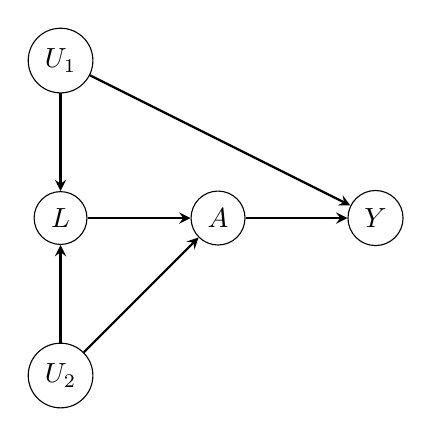
\begin{tikzpicture}
    \node[circle, draw] (L) at (-3, 0) {$L$};
    \node[circle, draw] (A) at (-1, 0) {$A$};
    \node[circle, draw] (Y) at (1, 0) {$Y$};
    \node[circle, draw] (U1) at (-3, 2) {$U_1$};
    \node[circle, draw] (U2) at (-3, -2) {$U_2$};

    \draw[-stealth, thick] (A) -- (Y);
    \draw[-stealth, thick] (L) -- (A);
    \draw[-stealth, thick] (U1) -- (L);
    \draw[-stealth, thick] (U2) -- (L);
    \draw[-stealth, thick] (U1) -- (Y);
    \draw[-stealth, thick] (U2) -- (A);
\end{tikzpicture}
\end{document}